\documentclass[10pt]{article}
\usepackage{fancyhdr, geometry, tikz}
\usetikzlibrary{positioning}
\pagestyle{fancy}

\lhead{\sf CS 6110 Homework 1}
\rhead{\sf Giang Nguyen (htn26) and Quinn Beightol (qeb2)}

\begin{document}
\subsection*{\sf 1 Free and Bound Variables}
  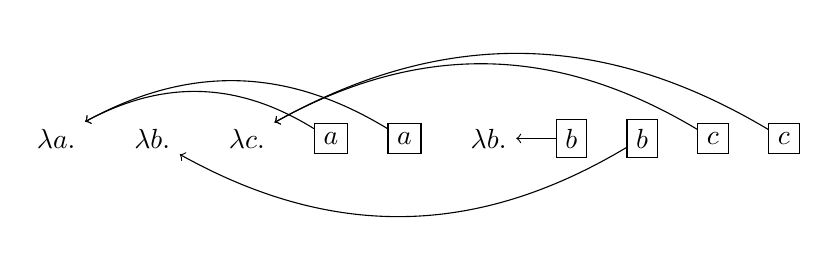
\begin{tikzpicture}[node distance=0.5cm]
    \node (absA) {$\lambda a.$};
    \node (absB1) [right=of absA] {$\lambda b.$};
    \node (absC) [right=of absB1] {$\lambda c.$};
    \node[rectangle, draw] (a1)    [right=of absC] {$a$};
    \node[rectangle, draw] (a2)   [right=of a1] {$a$};
    \node (absB2) [right=of a2] {$\lambda b.$};
    \node[rectangle, draw] (b1) [right=of absB2] {$b$};
    \node[rectangle, draw] (b2) [right= of b1] {$b$};
    \node[rectangle, draw] (c1) [right=of b2]{$c$};
    \node[rectangle, draw] (c2) [right=of c1]{$c$};
    \path[->]
      (a1) edge [bend right]  node {} (absA)
      (a2) edge [bend right]  node {} (absA)
      (b1) edge              node {} (absB2)
      (b2) edge [bend left] node {} (absB1)
      (c1) edge [bend right] node {} (absC)
      (c2) edge [bend right] node {} (absC);
  \end{tikzpicture}
\subsection*{\sf 2 Safe Substitution}
\subsection*{\sf 3 Small-Step Operational Semantics}
\subsection*{\sf 4 $\lambda$-Calculus Encodings}
\subsection*{\sf 5 $\lambda$-Calculus Programming}
\subsection*{\sf 6 Implementing the $\lambda$-Calculus}
\subsection*{\sf 7 Debriefing}
\end{document}
